\begin{frame}
\frametitle{Aircraft W\&B}
\begin{center}
Fixed-wing Aircraft Weight and Balance
\end{center}
\end{frame}

\begin{frame}
\frametitle{Fixed-wing Aircraft Weight and Balance}
\begin{block}{Basic principles}
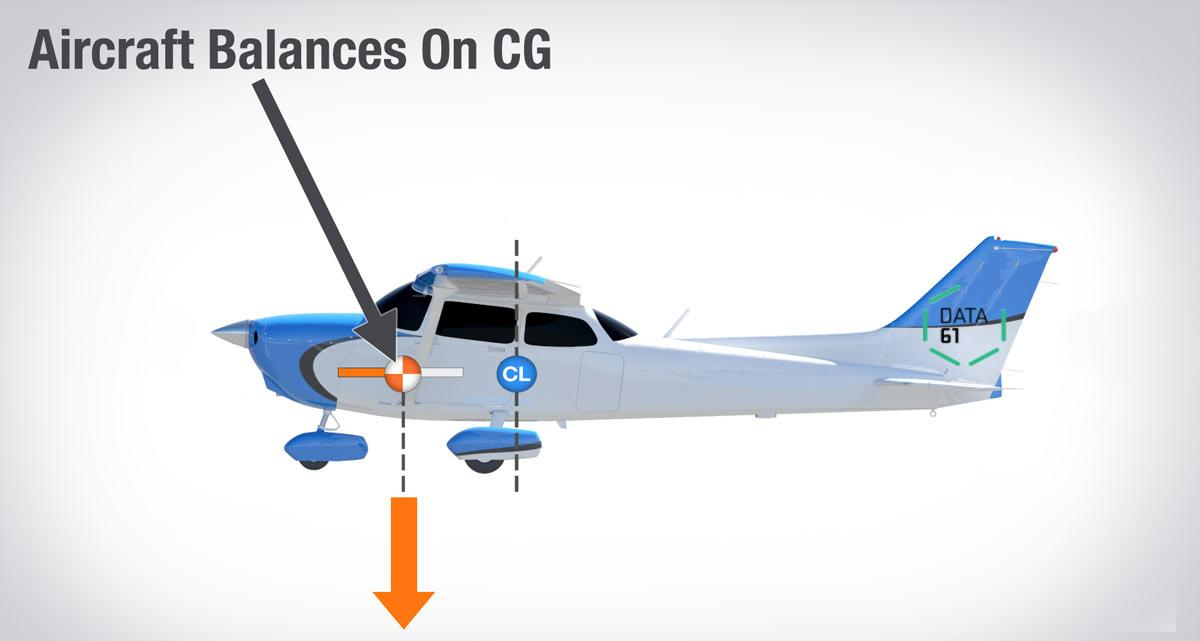
\includegraphics[height=0.5\textheight]{image/aircraft-cg.jpg}
\end{block}
\end{frame}

\begin{frame}
\frametitle{Fixed-wing Aircraft Weight and Balance}
\begin{block}{Same principles apply to A380}
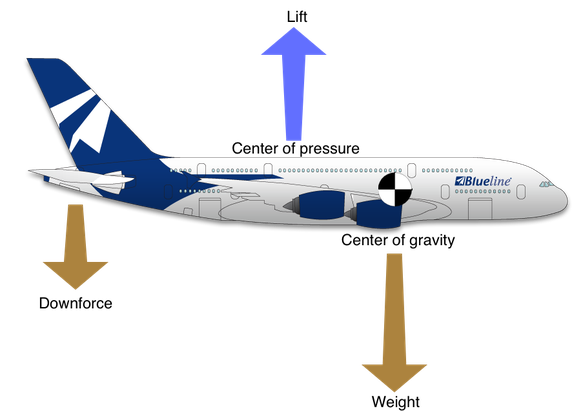
\includegraphics[height=0.5\textheight]{image/aircraft-cg-a380.png}
\end{block}
\end{frame}

\begin{frame}
\frametitle{Fixed-wing Aircraft Weight and Balance}
\begin{block}{Weight, Balance \emph{\tiny{loosely speaking}}}
\begin{itemize}
\item Weight is ensuring that the aircraft is not too heavy to maintain flight.
\item Balance is ensuring that the CG is positioned such that the aircraft is controllable.
\end{itemize}
\end{block}
\end{frame}

\begin{frame}
\frametitle{Fixed-wing Aircraft Weight and Balance}
\begin{block}{Calculating Weight and Balance}
\begin{itemize}
\item<1-> Obtain weights of front and rear PAX, baggage, fuel, aircraft itself.
\item<2-> Multiply each weight by a constant and plotting the results on a graph.
\item<3-> The final result is a yes/no to whether the point falls in an acceptable flight envelope for that aircraft.
\end{itemize}
\end{block}
\end{frame}
\begin{frame}

\frametitle{Fixed-wing Aircraft Weight and Balance}
\begin{block}{then this happens}
\begin{itemize}
\item<1-> Operator: ``We've changed your aircraft to VH-LSE.'' \emph{with a different empty weight}
\item<2-> Jessica: ``Hey is it cool if I sit in the front?''
\item<3-> I now have time pressure and distractions.
\item<3-> Start the calculation again, or use my previous calculations and declare the difference insignificant.
\end{itemize}
\end{block}
\end{frame}

\begin{frame}
\frametitle{Fixed-wing Aircraft Weight and Balance}
\begin{block}{I reject this compromise}
\begin{itemize}
\item<1-> My W\&B calculations are written in Haskell.
\item<2-> Jessica is a function argument and I can seat her anywhere, and immediately recalculate.
\item<3-> Different aircraft (and their weights) are function arguments.
\item<4-> Use diagrams package for producing the flight envelope plot.
\end{itemize}
\end{block}
\end{frame}

\begin{frame}
\frametitle{Fixed-wing Aircraft Weight and Balance}
\begin{block}{Example result}
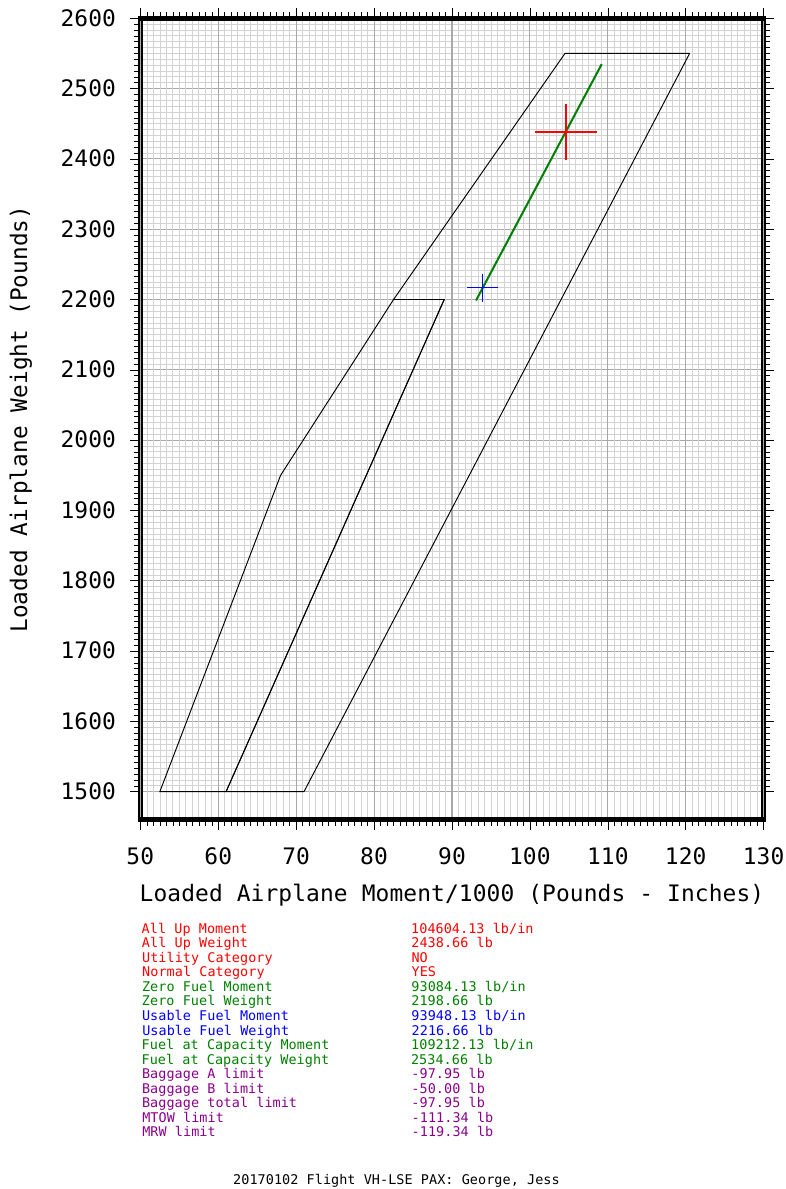
\includegraphics[height=0.6\textheight]{image/20170102-vhlse.png}
\end{block}
\end{frame}
